\documentclass[11pt]{article}

\usepackage[utf8]{inputenc}
\usepackage{array}
\usepackage{booktabs}   % For improved table formatting
\usepackage{tabulary}   % For tables with adjustable column widths
\usepackage{caption}
\usepackage{float}
\usepackage{amsmath}
\usepackage{amssymb}
\usepackage{tabularx}

\let\oldemptyset\emptyset
\let\emptyset\varnothing


\usepackage{amsmath} % For advanced math typesetting
\usepackage{pgfplots} % For creating graphs and plots
\pgfplotsset{compat=1.17} % Compatibility setting for pgfplots

\usepackage{graphicx} % For including graphics
\usepackage{float} % Helps to place figures and tables at precise locations

% Setting up the margins:
\usepackage[a4paper, total={6in, 8in}]{geometry}

% Improves the interface for defining floating objects such as figures and tables:
\usepackage{caption}
\usepackage{subcaption}

\title{Problem Set 7 - Unit VIII Sections 8.1 and 8.2}
\author{POL 201 - POL 501}
\date{\today}

\begin{document}
\maketitle

\section{Example: Estimating Linear Regression Parameters}

Assuming we have a dataset where:
\begin{itemize}
    \item \(X\): Number of public parks in a city
    \item \(Y\): Average life satisfaction score (scale of 100 points)
\end{itemize}

\subsection*{Data Points}
We consider the following 15 data points for \(X\) and \(Y\):
\[
\begin{array}{cc}
\hline 
    \text{X (Number of Parks)} & \text{Y (Life Satisfaction)} \\ \hline 
    2 & 68.97 \\
    5 & 68.62 \\
    4 & 74.48 \\
    8 & 91.23 \\
    3 & 63.66 \\
    10 & 77.66 \\
    6 & 87.79 \\
    7 & 81.67 \\
    12 & 79.31 \\
    1 & 67.43 \\
    3 & 61.37 \\
    11 & 77.34 \\
    9 & 80.42 \\
    4 & 48.87 \\
    2 & 46.75 \\ \hline 
\end{array}
\]

\subsection*{Calculations}
\begin{itemize}
    \item[(a)] Calculate the sample means (\(\overline{X}\) and \(\overline{Y}\)).
    \item[(b)] Calculate the sample variance of \(X\) (\(s_X^2\)) and the sample covariance between \(X\) and \(Y\) (\(s_{XY}\)).
    \item[(c)] Using the formulas derived in the theoretical framework, compute the regression coefficients \(\hat{\beta}\) and \(\hat{\alpha}\).
    \item[(d)] State the regression equation and interpret the results in the context of the problem.
    \item[(e)] Plot the data points and the regression line on a graph.
\end{itemize}


\section*{Solution}

\subsection*{Calculations}

\begin{itemize}
    \item[(a)] Calculate the sample means (\(\overline{X}\) and \(\overline{Y}\)):
    \[
    \overline{X} = \frac{1}{15} \sum_{i=1}^{15} X_i = 5.8
    \]
    \[
    \overline{Y} = \frac{1}{15} \sum_{i=1}^{15} Y_i = 71.70
    \]

    \item[(b)] Calculate the sample variance of \(X\) (\(s_X^2\)) and the sample covariance between \(X\) and \(Y\) (\(s_{XY}\)):
    \[
    s_X^2 = \frac{1}{14} \sum_{i=1}^{15} (X_i - \overline{X})^2 = 12.457
    \]
    \[
    s_{XY} = \frac{1}{14} \sum_{i=1}^{15} (X_i - \overline{X})(Y_i - \overline{Y}) = 28.808
    \]

    \item[(c)] Using the formulas derived in the theoretical framework, compute the regression coefficients \(\hat{\beta}\) and \(\hat{\alpha}\):
    \[
    \hat{\beta} = \frac{s_{XY}}{s_X^2} = \frac{28.808}{12.457} = 2.313
    \]
    \[
    \hat{\alpha} = \overline{Y} - \hat{\beta} \overline{X} = 71.70 - 2.313 \times 5.8 = 58.291
    \]

    \item[(d)] State the regression equation and interpret the results in the context of the problem:
    \[
    Y = 58.291 + 2.313X
    \]
    This equation implies that for each additional public park in the city, the average life satisfaction score increases by approximately 2.313 points.

    \item[(e)] Plot the data points and the regression line on a graph:

\begin{center}
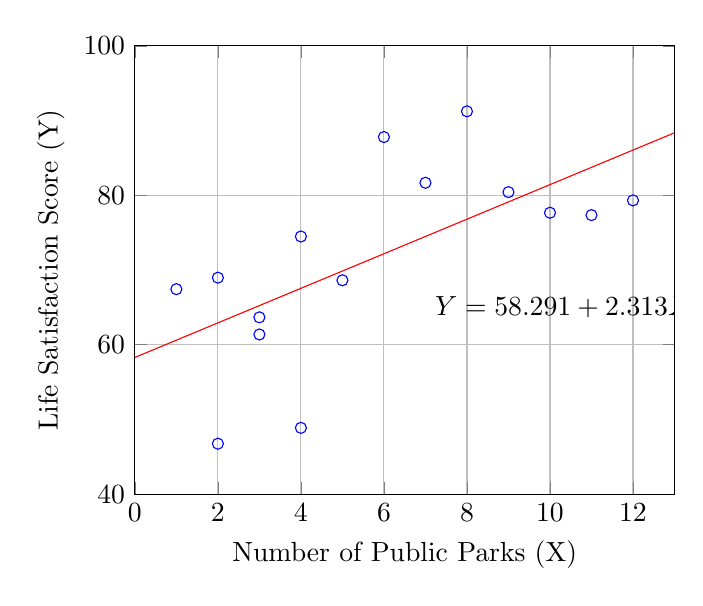
\begin{tikzpicture}
\begin{axis}[
    xlabel={Number of Public Parks (X)},
    ylabel={Life Satisfaction Score (Y)},
    xmin=0, xmax=13,
    ymin=40, ymax=100,
    grid=major,
    scatter/classes={
        a={mark=o,draw=blue}
    }
]

% Scatter plot
\addplot[scatter,only marks,scatter src=explicit symbolic]table[meta=label] {
x       y       label
2       68.97   a
5       68.62   a
4       74.48   a
8       91.23   a
3       63.66   a
10      77.66   a
6       87.79   a
7       81.67   a
12      79.31   a
1       67.43   a
3       61.37   a
11      77.34   a
9       80.42   a
4       48.87   a
2       46.75   a
};

% Regression line
\addplot[domain=0:13, samples=100, color=red]{58.291 + 2.313*x};

% Equation of the regression line
\node at (axis cs:7,65) [anchor=west] {$Y = 58.291 + 2.313X$};

\end{axis}
\end{tikzpicture}
\end{center}

\end{itemize}


\section{Example: Interpreting a Regression Line}

Assume you have conducted a study to analyze the relationship between the number of hours studied (\(X\)) and the score achieved on an exam (\(Y\)). The data has been collected, and the regression analysis resulted in the following linear regression equation:
\[
Y = 50 + 5X
\]
where \(Y\) is the exam score and \(X\) is the number of hours studied.

\subsection*{Problem}

\begin{itemize}
    \item[(a)] Interpret the meaning of the intercept in the context of this problem.
    \item[(b)] Interpret the meaning of the slope in the context of this problem.
    \item[(c)] If a student studied for 6 hours, predict their exam score using the regression equation.
    \item[(d)] Calculate the change in predicted exam score if the number of hours studied increases from 4 to 8 hours.
\end{itemize}

\section{Example: Interpreting a Linear Regression Line}

In many cases, the relationship between the independent variable \(X\) and the dependent variable \(Y\) can be modeled using a simple linear regression equation. This type of model assumes that \(Y\) changes at a constant rate as \(X\) changes.

Suppose a researcher is studying the effect of daily exercise duration (\(X\), in hours) on the fatigue level (\(Y\), on a scale from 0 to 100) experienced at the end of the day. The following regression equation was estimated:
\[
Y = 77 - 3.7X
\]
where \(Y\) is the fatigue level and \(X\) is the number of hours of exercise.

\subsection*{Problem}

\begin{itemize}
    \item[(a)] Interpret the meaning of the intercept in the context of this problem.
    \item[(b)] Interpret the meaning of the slope in the context of this problem.
    \item[(c)] If a person exercises for 2 hours, predict their fatigue level using the regression equation.
    \item[(d)] Calculate the predicted change in fatigue level when the exercise duration increases from 1 hour to 3 hours.
    \item[(e)] Plot the regression line for \(X\) values ranging from 0 to 10 hours.
\end{itemize}

\section{Open Question: Discuss the following assumptions related to Simple Linear Regression:}
        \begin{itemize}
            \item[(i)] Explain what is the linearity assumption in SLR.
            \item[(ii)] Explain what is the assumption of conditional independence between \(X\) and \(\epsilon\).
            \item[(iii)] Explain the assumption of zero mean for \(\epsilon\).
        \end{itemize}

\section{Example: Estimating and Interpreting Regression Coefficients}

A researcher is analyzing the relationship between hours of study per week (\(X\)) and test scores (\(Y\)) among students. The following table provides summary statistics based on a sample of 30 students:

\[
\begin{array}{|c|c|}
\hline
\text{Statistic} & \text{Value} \\
\hline
\text{Mean of } X, \overline{X} & 10 \\
\text{Mean of } Y, \overline{Y} & 75 \\
\text{Variance of } X, s_X^2 & 16 \\
\text{Variance of } Y, s_Y^2 & 49 \\
\text{Covariance between } X \text{ and } Y, s_{XY} & 11.2 \\
\text{Correlation coefficient between } X \text{ and } Y, r_{XY} & 0.4 \\
\hline
\end{array}
\]

Based on this information, answer the following questions:

\subsection*{Problem}

\begin{itemize}
    \item[(a)] Compute the estimates of the regression coefficients \(\alpha\) and \(\beta\) in the linear regression model \(Y = \alpha + \beta X\). Use the formulas:
    \[
    \hat{\beta} = \frac{s_{XY}}{s_X^2}, \quad \hat{\alpha} = \overline{Y} - \hat{\beta} \overline{X}
    \]
    \item[(b)] Interpret the estimates of \(\alpha\) and \(\beta\) in the context of the problem. What do they tell you about the relationship between hours of study and test scores?
    \item[(c)] Plot the regression line based on your estimates along with the data points. Assume the data points are centered around the means provided, with \(X\) ranging from 5 to 15 hours.
\end{itemize}

\section{Example: Estimating Linear Regression Parameters}

Assuming we have a dataset where:
\begin{itemize}
    \item \(X\): Time spent on social media per day (hours)
    \item \(Y\): Productivity score (scale of 100 points)
\end{itemize}

\subsection*{Data Points}
We consider the following 8 data points for \(X\) and \(Y\):
\[
\begin{array}{|c|c|}
\hline 
    \text{X (Hours on Social Media)} & \text{Y (Productivity Score)} \\ \hline 
    1.0 & 51.01 \\
    2.0 & 28.74 \\
    3.0 & 21.09 \\
    4.0 & 18.44 \\
    5.0 & 5.40 \\
    6.0 & 2.81 \\
    7.0 & 10.31 \\
    8.0 & 5.30 \\ \hline 
\end{array}
\]

\subsection*{Calculations}
\begin{itemize}
    \item[(a)] Calculate the sample means (\(\overline{X}\) and \(\overline{Y}\)).
    \item[(b)] Calculate the sample variance of \(X\) (\(s_X^2\)) and the sample covariance between \(X\) and \(Y\) (\(s_{XY}\)).
    \item[(c)] Using the formulas derived in the theoretical framework, compute the regression coefficients \(\hat{\beta}\) and \(\hat{\alpha}\).
    \item[(d)] State the regression equation and interpret the results in the context of the problem.
    \item[(e)] Plot the data points and the regression line on a graph.
\end{itemize}


\end{document}
